\section{Introduzione}

\subsection{Descrizione del problema}
In questa relazione illustreremo dei confronti tra due algoritmi per risolvere il problema del \textit{Minimum Cut}, confrontando i tempi di calcolo e la correttezza delle soluzioni trovate. \\
Quello del \textit{Minimum Cut} è un problema di ottimizzazione che può essere definito come segue:
\begin{center}
    \centering
    \textit{
        Dato un multigrafo $\mathcal{G}=(\mathcal{V}, \mathcal{E})$, trovare un insieme $\mathcal{E}{}'\subseteq \mathcal{E}$ tale che $\mathcal{E}{}'$ sia minimo,\\ ossia contenga il minor numero di archi.
    }
\end{center}
Nel caso specifico di questo laboratorio, il problema è stato esteso a grafi pesati; il problema diventa pertanto trovare l'insieme di lati da rimuovere da un grafo in modo tale che la somma dei pesi di questi sia minima. \\
Per risolvere questo problema abbiamo implementato due algoritmi: l'algoritmo di \textit{Stoer e Wagner} e l'algoritmo di \textit{Karger e Stein}. Nello specifico, il primo è un algoritmo deterministico, mentre il secondo è un algoritmo randomizzato.

\subsection{Definizioni utili}

\subsubsection*{Multigrafo non orientato}
Un \textit{multigrafo} è un grafo $\mathcal{G}=(\mathcal{V}, \mathcal{E})$ tale che $\mathcal{V} \subseteq \mathbb{N}$, con $\mathcal{V}$ finito, e $\mathcal{E}$ è un multiinsieme a elementi del tipo $\{u, v\}: u\neq v$

\subsubsection*{Cammino in un multigrafo}
Un \textit{cammino in un multigrafo} consiste in una sequenza di nodi $\{v_1, v_2, ..., v_t\}$ dove per ogni coppia di nodi $\{v_i, v_{i+1}\}$ esiste un lato $e_j$ che li unisce.

\subsubsection*{Connettività di un multigrafo}
Un multigrafo è \textit{connesso} se per ogni coppia di nodi $v_i, v_j$ esiste un cammino che li connette.

\subsubsection*{Taglio}
Dato $\mathcal{G}=(\mathcal{V}, \mathcal{E})$ un multigrafo connesso, un \textit{taglio} $\mathcal{C} \subseteq \mathcal{E}$ è un multiinsieme di lati tale che $\mathcal{G}{}'=(\mathcal{V}, \mathcal{E}-\mathcal{C})$ non è connesso o, equivalentemente, $\mathcal{G}{}'$ ha almeno due componenti connesse.

\subsubsection*{Contrazione di un multigrafo rispetto ad \textit{e}}
Dato $\mathcal{G}=(\mathcal{V}, \mathcal{E})$ un multigrafo ed $e=\{u,v\} \in \mathcal{E}$, la \textit{contrazione} di $\mathcal{G}$ rispetto ad $e$, $\mathcal{G}/e=(\mathcal{V}{}', \mathcal{E}{}')$ è il multigrafo con:
\begin{itemize}
    \item[] $\mathcal{V}{}'=\mathcal{V} \setminus \{u, v\} \cup \{z_{u,v}\}$
    \item[] $\mathcal{E}{}'=\mathcal{E} \setminus \{\{\{x, y\}: (x=u) \vee (x=v)\}\} \cup \{\{\{z_{u,v}, y\}: (\{u,y\} \in \mathcal{E}) \vee (\{v,y\} \in \mathcal{E}), (y\neq u) \wedge (y \neq v) \}\}$
\end{itemize}
Viene riportato di seguito un esempio grafico di contrazione di un multigrafo rispetto a un arco.

\begin{figure}[H]
	\centering
	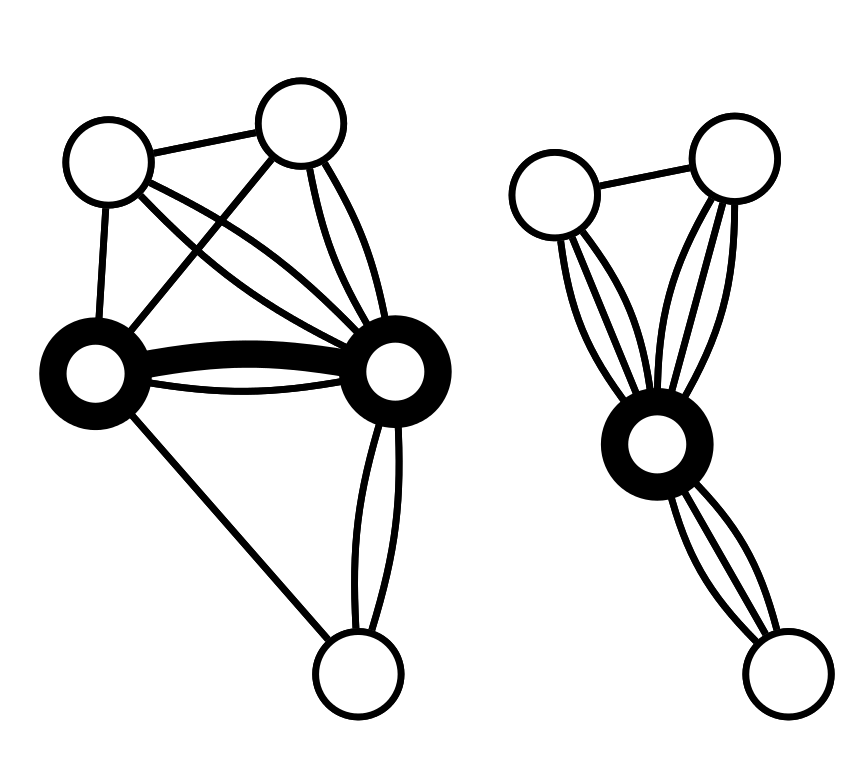
\includegraphics[width=0.5\textwidth]{res/images/multigraph}
	\caption{Esempio di contrazione di un multigrafo.}
	\label{fig:multigraph_contraction}
\end{figure}